\section{Results}

%read Willis et al., 2010 and Willis and Fortey, 2003 on use of paleontological data.

% read Thompson and Withers, 2003: Species Accumulation Curve
\subsection{Sample-based accumulation curves}
The sample-based accumulation curve (SAC) on the generic level shows a relatively low intial slope and a long upward slope to the asymptote, which does not reach full saturation (Fig. \ref{fig:SACGen}).
%Although the SAC does not completely plateau, considering the large area covered and the high number of rare genera in the dataset, it can be considered well enough sampled for our purposes.
In contrast, the species accumulation curves, both per reference and per locality, show only a slight initial increase and, for the same number of references/sampling units, are far from reaching an asymptote (Fig. \ref{fig:SACall} (a), (b)).
% DISCUSSION: as could be expected, since there are less genera than species \citep{Gotelli2001}. At a large geographic scale, it can be expected, that an asymptote is not reached \citep{Thompson2002}. Fig. \ref{fig:SACGen} corresponds to the shape one would expect, when there are many genera that are rare and only a few abundant ones. For the different continents, only Europe and Eurasia show some sort of "typical" SAC shape.
%%%____
% DISCUSSION ? 
%Since there are less genera than species, it is to be expected that genera reach an asymptote earlier than species.
%%%____
Accumulation curves for individual continents show that Europe reflects the trend of the overall dataset, with a long upward slope after the inflection point, whereas the other continents require further sampling (Fig. \ref{fig:SACall} (c) - (i)). For this reason, the timescale analysis was only conducted for Europe and Eurasia, but not for the other continents.

%--> genera sufficiently sampled, species not
%--> for genera, when splitting up continents only Europe and Eurasia are sampled well enough --> ask Johannes again, I feel like Asia is screwing up the results, would stick with Europe.
%--> maybe refer to table 20: overview over fossil genera per time bin??

%_______________________________________________________________________
\begin{figure}[htbp]
	\centering
	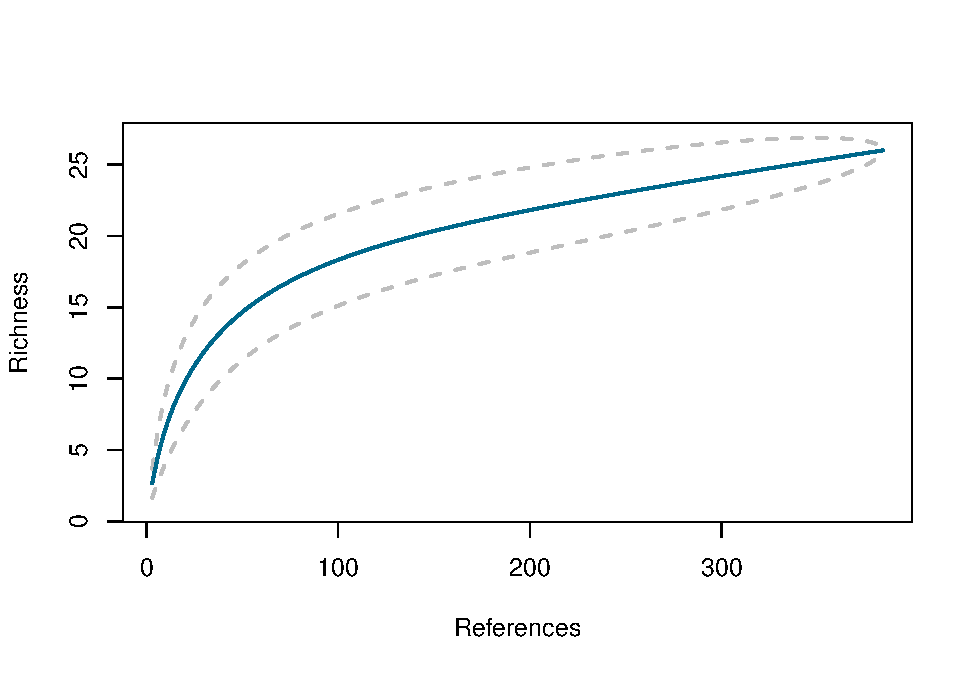
\includegraphics[width=0.8\textwidth]{MA_JJ_files/figure-latex/SACGenera-1.pdf}
	\caption[Sample-based accumulation curve on generic level]{Sample-based accumulation curve of fossil genera per reference. Dashed lines represent the confidence inteval.}
	\phantomsection
	\label{fig:SACGen}
\end{figure}


\FloatBarrier


%read: Smith and Lyons, 2010 (?) and Smith et al., 2016
%--> body size patterns (see also table 22, general statistics)

%data is bimodal (not normally distributed --> fig. ), still visible in pretty much all subgroups that you could split them into.
%as most animal groups/clades (?) right-skewed = smaller body size more frequent, BUT island species are left-skewed with more larger body sizes! (logtransformed data, skewness: negative for Zanclean, Messinian ??, insular, fossil-insular, but not modern-insular!!)
\subsection{Descriptive statistics}

The histograms indicate that testudinid body size is not normally distributed (Fig. \ref{fig:histAll}), which is supported by QQ-Plots for raw as well as log-transformed data (Fig. \ref{fig:NormDis}).

The body size distribution is moderately right-skewed (Table \ref{tab:stats}), with a higher frequency of smaller body sizes.
Body size ranges from a minimum of 80 mm to a maximum of 2500 mm for the entire data set. When comparing body sizes on a temporal scale, the minimum body size per stratigraphic stages excluding modern taxa ranges from 90 mm to 270 mm, while the maximum 1100 mm to 2500 mm. The highest maximum body size was observed in the fossil record from continental Europe (CL = 2500 mm).
%________________________________________________________________________

\begin{figure}[htbp]
	\centering
	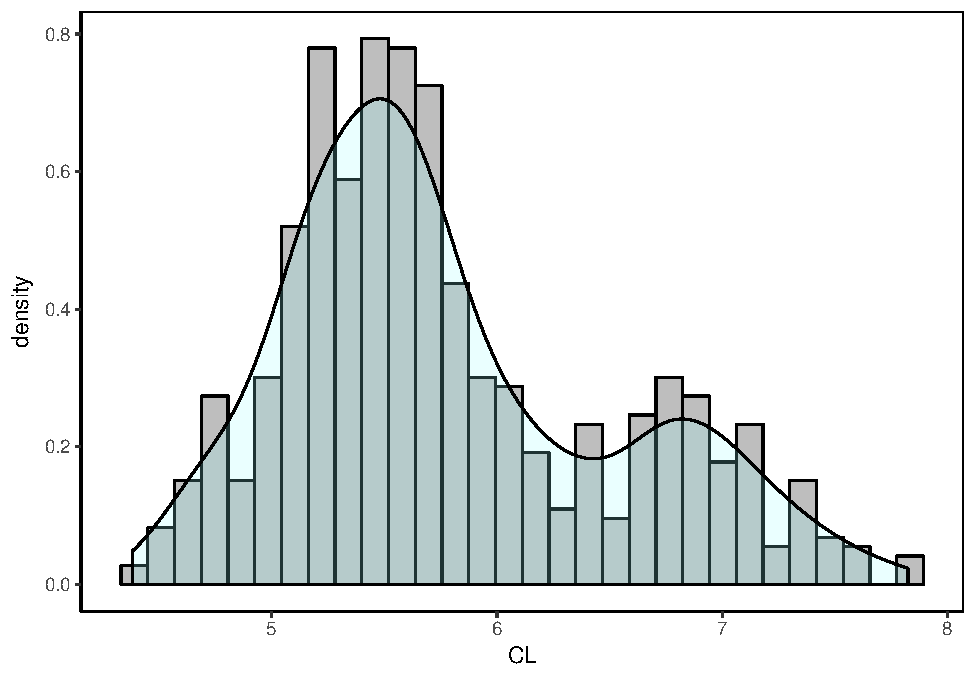
\includegraphics[width=0.8\textwidth]{MA_JJ_files/figure-latex/HistAll-1.pdf}
	\caption[Body size distribution of complete data set]{Body size distribution of complete data set. The data is bimodally distributed and right-skewed.}
	\phantomsection
	\label{fig:histAll}
\end{figure}

This pattern is also apparent when splitting the data set into fossil and modern taxa (Fig. \ref{fig:HistFMCI} (a)). Considering insularity, body size distribution is right-skewed for continental taxa, but left-skewed for insular species, meaning larger body size is more frequent than smaller body size on islands. Insular taxa are also left-skewed when only considering fossil taxa, but modern insular taxa have a skewness close to 0, indicating a symmetric distribution (Table \ref{tab:stats}).
Kurtosis suggests light tails with no/few outliers (kurtosis < 3) for insular and modern insular species, whereas continental species have a heavy tail (kurtosis > 3; Table \ref{tab:stats}).

\begin{center}
	\begin{figure}[htbp]
		\subfloat[Fossil vs. modern]{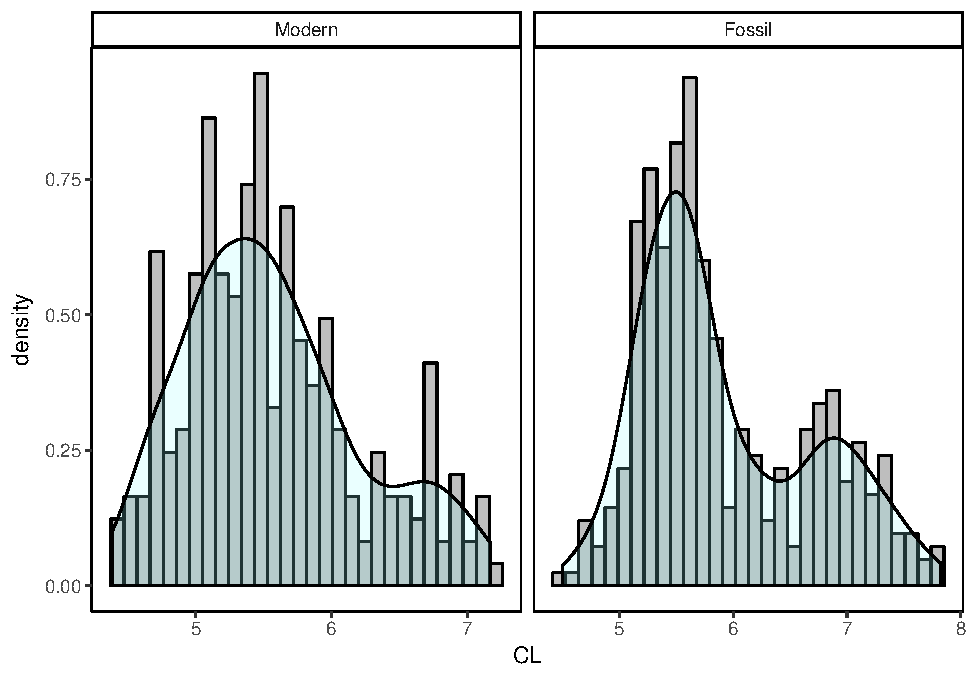
\includegraphics[scale=0.45]{MA_JJ_files/figure-latex/HistFosMo-1.pdf}}
		\subfloat[Continental vs. insular]{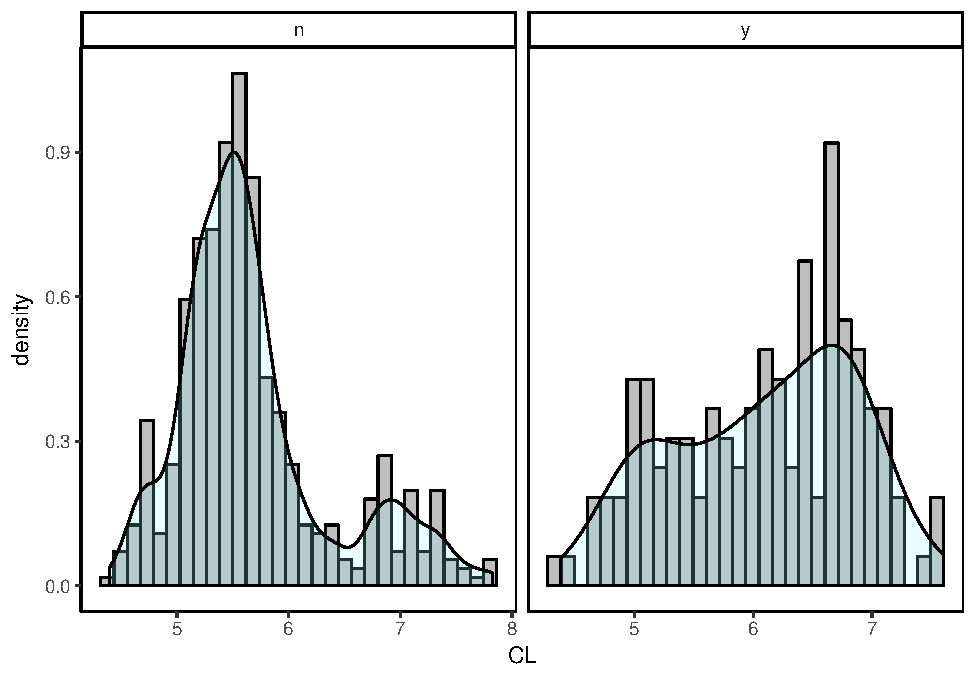
\includegraphics[scale=0.45]{MA_JJ_files/figure-latex/HistCI-1.pdf}}	
		\caption[Body size distribution comparing fossil/modern and continental/insular taxa.]{Comparison of body size distributions of modern vs. fossil and continental vs. insular data. All distributions are bimodal. Fossil, modern and continental subgroups are right-skewed whereas the distribution of insular data is left-skewed.}
		\phantomsection
		\label{fig:HistFMCI}
	\end{figure}
\end{center}

The histograms show a bimodal distribution, wich is also apparent on most sublevels, except for modern insular species (Fig. \ref{fig:HistRest} (a)).
Body size distributions are similar, right-skewed and bimodal, for the four continents and reflect the overall trend (Fig. \ref{fig:HistRest} (b)).




\FloatBarrier

%__________________________



Mean body size differs significantly across time bins (Kruskal Wallis Test, $\chi^2$ = 71.441, P < 0.01; Fig. \ref{fig:boxBins}). 
The multiple comparison test showed that modern median body size is smaller than body size in the Upper Pleistocene. %(Wilcoxon Rank Sum Test, W = 3853.5, P < 0.01 )
There is no difference in body size within the Pleistocene %(Wilcoxon Rank Sum Test, P > 0.05)
and Pleistocene body size does not differ from body size in the Upper Miocene%(Wilcoxon Rank Sum Test, P > 0.05)
. Serravallian body size is smaller than Langhian body size in the Middle Miocene%(Wilcoxon Rank Sum Test, W = 45, P < 0.01)
, but Langhian body size is not different from Lower Miocene body size%(Wilcoxon Rank Sum Test, W = 311, P = 0.06)
.


%__________________________________________________________________________
\begin{figure}[hbtp]
	\centering
	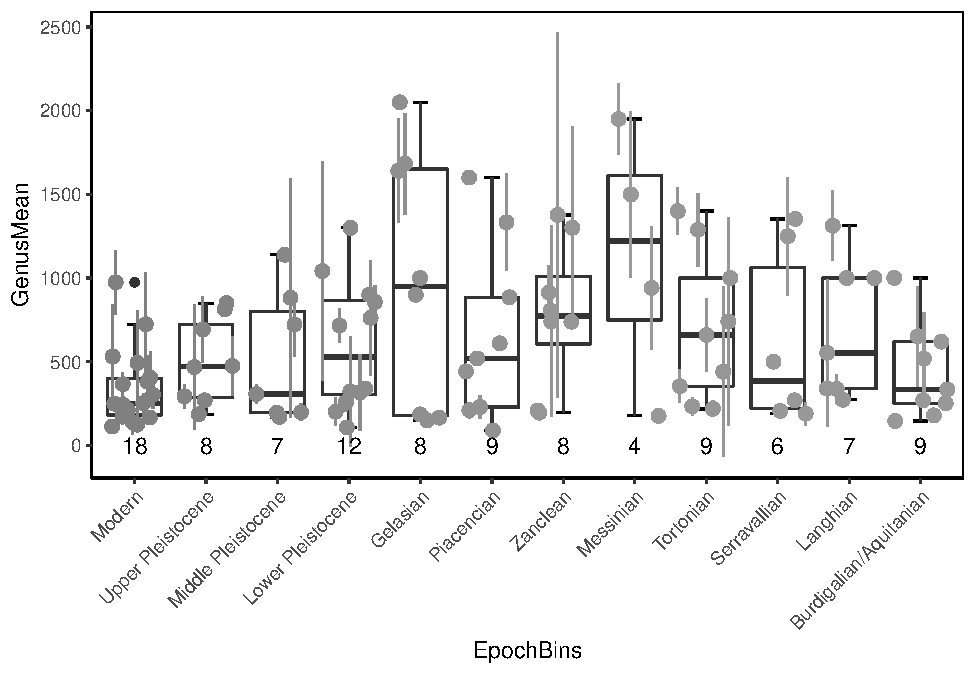
\includegraphics[width=0.9\textwidth]{MA_JJ_files/figure-latex/BPGBins-1.pdf}
	\caption[Comparison of carapace length across time bins]{Comparison of carapace length across all time bins. Bold lines indicate medians, boxes indicate lower and upper quartiles, whiskers indicate largest and smallest observations and outliers represent extreme values. Numbers refer to number of genera per time bin. The mean carapace lengths per genera are depicted as grey circles with errorbars indicating the respective standard deviation. Smallest average carapace length and variance is found in modern testudinids.}
	\phantomsection
	\label{fig:boxBins}
\end{figure}

%\todo{random sampling necessary?}
% = 71.441, df = 11, p-value = 6.496e-11


%need statistics for boxplot!! kruskal-wallis-test plus post-hoc test (+ bonferroni correction?) or moving mean (faysal?)
%you can kind of see how the median increases and then decreases again
%(compare in order: Modern < Upper Pleistocene etc., do median and variance??)

% FOR ALL TIME STAGES

%	Kruskal-Wallis rank sum test

%data:  list(M, UPle, MPle, LPle, G, Pia, Z, Mess, Tort, S, L, BA)
%Kruskal-Wallis chi-squared = 71.441, df = 11, p-value = 6.496e-11

%Multiple comparison test after Kruskal-Wallis 
%p.value: 0.05 
%Comparisons
%obs.dif critical.dif difference
%Modern-Upper Pleistocene                  116.987013     93.54915       TRUE
%Modern-Middle Pleistocene                  80.140652     90.54349      FALSE
%Modern-Lower Pleistocene                   66.123604     87.87753      FALSE
%Modern-Gelasian                             1.627566    114.05459      FALSE
%Modern-Piacencian                         113.296537    136.11314      FALSE
%Modern-Zanclean                           205.945804    123.43828       TRUE
%Modern-Messinian                          137.122727    193.24680      FALSE
%Modern-Tortonian                           61.739394     96.96976      FALSE
%Modern-Serravallian                        21.764310    121.34770      FALSE
%Modern-Langhian                           202.487013    164.56067       TRUE
%Modern-Burdigalian/Aquitanian              70.472727    115.73561      FALSE
%Upper Pleistocene-Middle Pleistocene       36.846361    118.78423      FALSE
%Upper Pleistocene-Lower Pleistocene        50.863409    116.76486      FALSE
%Upper Pleistocene-Gelasian                115.359447    137.55006      FALSE
%Upper Pleistocene-Piacencian                3.690476    156.32773      FALSE
%Upper Pleistocene-Zanclean                 88.958791    145.42551      FALSE
%Upper Pleistocene-Messinian                20.135714    207.98052      FALSE
%Upper Pleistocene-Tortonian                55.247619    123.75260      FALSE
%Upper Pleistocene-Serravallian            138.751323    143.65527      FALSE
%Upper Pleistocene-Langhian                 85.500000    181.63641      FALSE
%Upper Pleistocene-Burdigalian/Aquitanian   46.514286    138.94713      FALSE
%Middle Pleistocene-Lower Pleistocene       14.017047    114.37094      FALSE
%Middle Pleistocene-Gelasian                78.513086    135.52379      FALSE
%Middle Pleistocene-Piacencian              33.155885    154.54785      FALSE
%Middle Pleistocene-Zanclean               125.805152    143.51048      FALSE
%Middle Pleistocene-Messinian               56.982075    206.64601      FALSE
%Middle Pleistocene-Tortonian               18.401258    121.49644      FALSE
%Middle Pleistocene-Serravallian           101.904962    141.71632      FALSE
%Middle Pleistocene-Langhian               122.346361    180.10681      FALSE
%Middle Pleistocene-Burdigalian/Aquitanian   9.667925    136.94153      FALSE
%Lower Pleistocene-Gelasian                 64.496038    133.75738      FALSE
%Lower Pleistocene-Piacencian               47.172932    153.00123      FALSE
%Lower Pleistocene-Zanclean                139.822200    141.84356      FALSE
%Lower Pleistocene-Messinian                70.999123    205.49188      FALSE
%Lower Pleistocene-Tortonian                 4.384211    119.52289      FALSE
%Lower Pleistocene-Serravallian             87.887914    140.02804      FALSE
%Lower Pleistocene-Langhian                136.363409    178.78144      FALSE
%Lower Pleistocene-Burdigalian/Aquitanian    4.349123    135.19364      FALSE
%Gelasian-Piacencian                       111.668971    169.39706      FALSE
%Gelasian-Zanclean                         204.318238    159.39129       TRUE
%Gelasian-Messinian                        135.495161    217.97454      FALSE
%Gelasian-Tortonian                         60.111828    139.89893      FALSE
%Gelasian-Serravallian                      23.391876    157.77782      FALSE
%Gelasian-Langhian                         200.859447    192.99946       TRUE
%Gelasian-Burdigalian/Aquitanian            68.845161    153.50345      FALSE
%Piacencian-Zanclean                        92.649267    175.85199      FALSE
%Piacencian-Messinian                       23.826190    230.28513      FALSE
%Piacencian-Tortonian                       51.557143    158.39839      FALSE
%Piacencian-Serravallian                   135.060847    174.39088      FALSE
%Piacencian-Langhian                        89.190476    206.80215      FALSE
%Piacencian-Burdigalian/Aquitanian          42.823810    170.53342      FALSE
%Zanclean-Messinian                         68.823077    223.02794      FALSE
%Zanclean-Tortonian                        144.206410    147.64914      FALSE
%Zanclean-Serravallian                     227.710114    164.68880       TRUE
%Zanclean-Langhian                           3.458791    198.68908      FALSE
%Zanclean-Burdigalian/Aquitanian           135.473077    160.59847      FALSE
%Messinian-Tortonian                        75.383333    209.54137      FALSE
%Messinian-Serravallian                    158.887037    221.87771      FALSE
%Messinian-Langhian                         65.364286    248.16258      FALSE
%Messinian-Burdigalian/Aquitanian           66.650000    218.85882      FALSE
%Tortonian-Serravallian                     83.503704    145.90588      FALSE
%Tortonian-Langhian                        140.747619    183.42158      FALSE
%Tortonian-Burdigalian/Aquitanian            8.733333    141.27276      FALSE
%Serravallian-Langhian                     224.251323    197.39708       TRUE
%Serravallian-Burdigalian/Aquitanian        92.237037    158.99725      FALSE
%Langhian-Burdigalian/Aquitanian           132.014286    193.99761      FALSE


% FOR MODERN - PLEISTOCENE - PLIOCENE - MIOCENE
%Kruskal-Wallis rank sum test

%data:  list(Modern, Plei, Plio, Mio)
%Kruskal-Wallis chi-squared = 37.764, df = 3, p-value = 3.172e-08


%Multiple comparison test after Kruskal-Wallis 
%p.value: 0.05 
%Comparisons
%obs.dif critical.dif difference
%Modern-Pleistocene   110.904114     49.80480       TRUE
%Modern-Pliocene       67.623302     58.35513       TRUE
%Modern-Miocene        64.510137     49.57182       TRUE
%Pleistocene-Pliocene  43.280812     64.36704      FALSE
%Pleistocene-Miocene   46.393977     56.52575      FALSE
%Pliocene-Miocene       3.113165     64.18694      FALSE



%__________________________________________________________________________
\begin{center}
	\begin{figure}[htbp]
		\subfloat[Modern testudinids have a smaller average carapace length and variance than their fossil counterparts.]{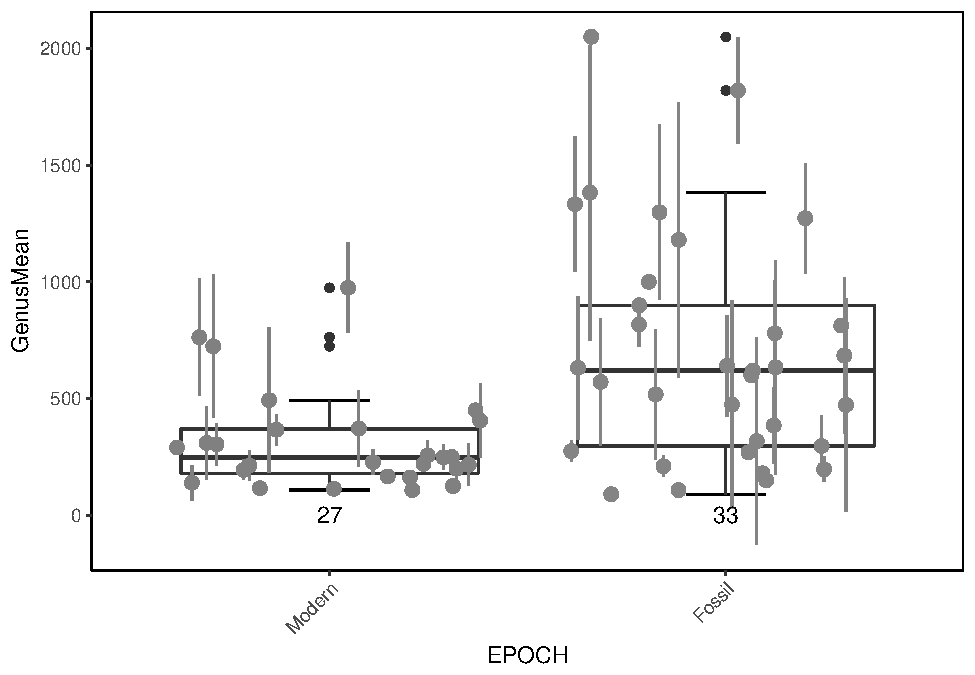
\includegraphics[scale=0.45]{MA_JJ_files/figure-latex/BPMF-1.pdf}}
		\subfloat[Continental \T have a larger average carapace length and variance than insular testudinids]{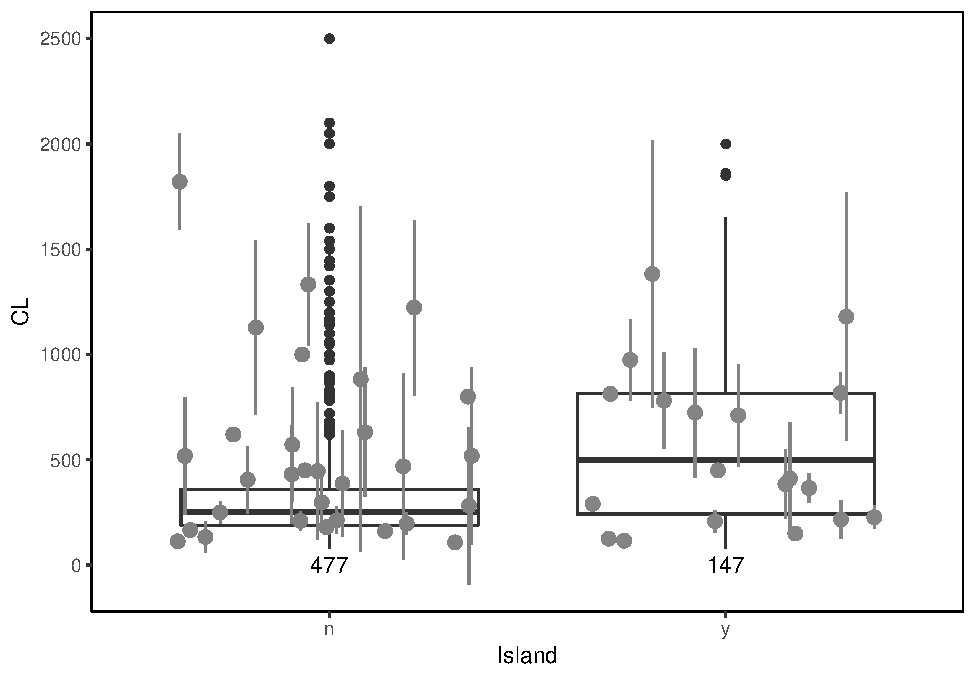
\includegraphics[scale=0.45]{MA_JJ_files/figure-latex/BPCI-1.pdf}}
		\caption[Comparing carapace lengths between fossil/modern and continental/insular testudinids]{Comparison of carapace length between (a) fossil and modern as well as (b) continental and insular testudinids. Bold lines indicate medians, boxes indicate lower and upper quartiles, whiskers indicate largest and smallest observations and outliers represent extreme values. Numbers refer to number of genera per time bin. The mean carapace lengths per genera are depicted as grey circles with errorbars indicating the respective standard deviation.}
		\phantomsection
		\label{fig:boxFMCI}
	\end{figure}
\end{center}



Comparison of modern and fossil testudinids showed that modern tortoises are significantly smaller than fossil ones (Wilcoxon Rank Sum Test, W = 22318, P < 0.01; Fig. \ref{fig:boxFMCI}). Furthermore, continental testudinids are significantly smaller than insular taxa (Wilcoxon Rank Sum Test, W = 13854, P < 0.01; Fig. \ref{fig:boxFMCI}).


\begin{figure}[htbp]
	\centering
	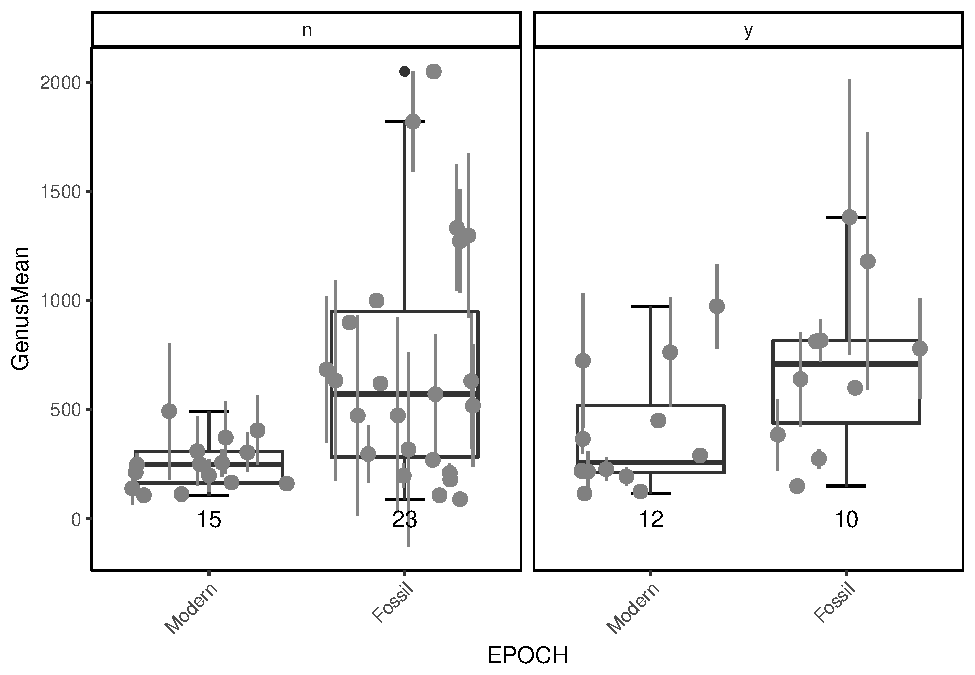
\includegraphics[width=0.75\textwidth]{MA_JJ_files/figure-latex/BPFMCI-1.pdf}
	\caption[Comparison of continental and insular testudinids of modern and fossil age]{Boxplots fossil vs.~modern, continental vs.~insular species.
		Comparison of carapace length among continental and insular \T of different age. Bold lines indicate medians, boxes indicate lower and upper quartiles, whiskers indicate largest and smallest observations and outliers represent extreme values. Numbers refer to number of genera per time bin. The mean carapace lengths per genera are depicted as grey circles with errorbars indicating the respective standard deviation. Modern testudinids are smaller than fossil ones both on continents and on islands.}
	\label{BoxFoMCI}
\end{figure}



These results can even be considered in combination: modern continental taxa are smaller than fossil continental taxa (Wilcoxon Rank Sum Test, W = 8046, P < 0.01; Fig. \ref{BoxFoMCI}) and modern insular taxa are smaller than fossil insular taxa (Wilcoxon Rank Sum Test, W = 631.5, P < 0.01; Fig. \ref{BoxFoMCI}))


\begin{figure}[htbp]
	\centering
	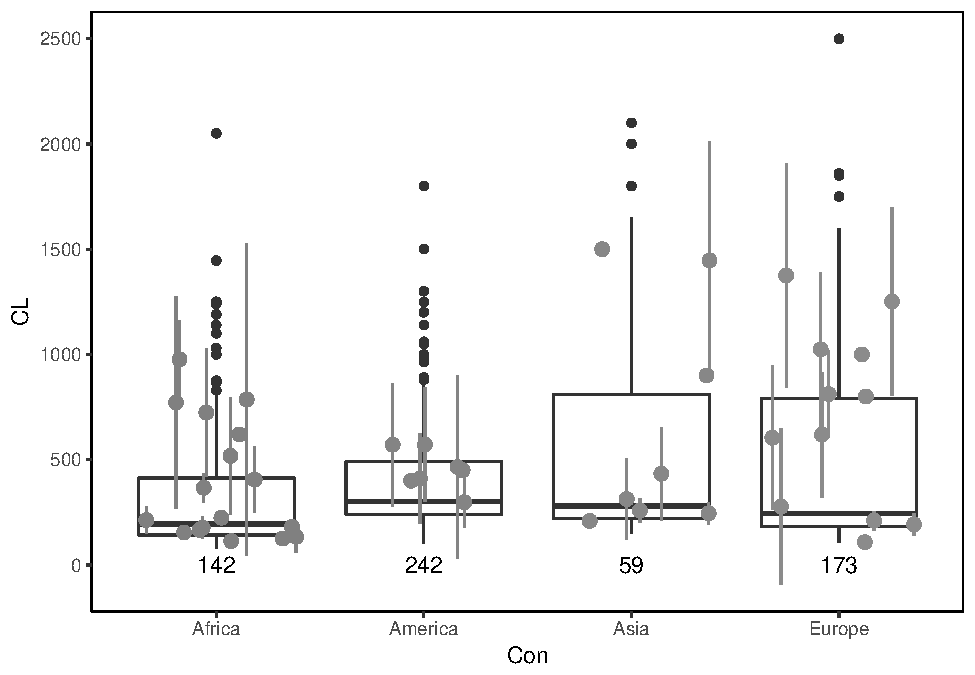
\includegraphics[width=0.75\textwidth]{MA_JJ_files/figure-latex/BPCon-1.pdf}
	\caption[Comparison of carapace lengths amon continents.]{Comparison of testudinid carapace length among continents. Bold lines indicate medians, boxes indicate lower and upper quartiles, whiskers indicate largest and smallest observations and outliers represent extreme values. Numbers refer to number of genera per time bin. The mean carapace lengths per genera are depicted as grey circles with errorbars indicating the respective standard deviation. African testudinids have the smallest average carapace length compared to the other continents.}
	\phantomsection
	\label{fig:boxCon}
\end{figure}




Finally, body size differs among continents (Kruskal Wallis Test, $\chi^2$ = 34.343, P < 0.01; Fig. \ref{fig:boxCon}). The multiple comparison test showed that African testudinids differ significantly from the other three continents in body size. American testudinid body size is comparable to that of Asia, but differs from those of Africa and Europe. Furthermore, Asian and European testidinids are similar in body size. %Since only Europe/Eurasia are well sampled, these relationships could change with further sampling. ??



\FloatBarrier
%__________________________________________________________________________

\subsection{paleoTS analysis}\label{paleots-analysis}


\subsubsection{complete dataset}\label{all-continental-and-insular}

How mean body size progresses over time is similar for the complete data set as well as continental and insular subgroups. All show peaks in the Upper Miocene and Lower Pleistocene and dip during the Pliocene. However, the decline in body size is very pronounced for continental testudinids, whereas body size only slowly decreases on islands. All three data sets also show a very sharp decline in the youngest time bin.
For the complete data set as well as the continental one, body size seems to increase constantly during the Miocene. For the insular data set, the Upper Miocene is the starting point for the analysis, but mean carapace length is even larger than on continents.
The model fittings showed that stasis is best supported for both the complete and the insular data set. However, while is very well supported for insular testudinids (100\,\%), the model support for the complete data set is rather weak (50\,\%). In conrast, on continents an unbiased random walk is the best supported model, but also with only a rather weak support.\\

Fitting of the three evolutionary models favoured stasis for the entire data set, although model support was only 51\,\% followed by 33\,\% support for the unbiased random walk (Fig. \ref{fig:pTSall}, Table \ref{tab:pTSall}). When solely considering continental genera, the best-fitting model was the unbiased random walk, but again not ideally supported with 55\,\% followed by a modest model support of 30\,\% for generalized random walk (Fig. \ref{fig:pTSC}, Table \ref{tab:pTSCEM}). In contrast, insular genera are best described by stasis, which was very well supported (100\,\%; Fig. \ref{fig:pTSI}, Table \ref{tab:pTSIEM})). 

\begin{longtable}[]{@{}rrrr@{}}
	\caption[PaleoTS object of complete dataset]{PaleoTS object of the complete data set. Mean Age (tt), sample size (nn), mean carapace lengths (mm) and variance (vv) are shown. Largest mean carapace length occurs in the Upper Miocene, followed by the Lower Pleistocene.}
	\phantomsection
	\label{tab:pTSall}\tabularnewline
	\toprule
	tt & nn & mm & vv\tabularnewline
	\midrule
	\endfirsthead
	\toprule
	tt & nn & mm & vv\tabularnewline
	\midrule
	\endhead
	0.00585 & 22 & 330.1456 & 50307.87\tabularnewline
	0.06885 & 8 & 506.3265 & 64620.11\tabularnewline
	0.45350 & 7 & 516.4053 & 155241.85\tabularnewline
	1.29350 & 12 & 593.8669 & 147507.20\tabularnewline
	2.19700 & 8 & 971.8850 & 580540.76\tabularnewline
	3.09400 & 9 & 658.0826 & 271043.73\tabularnewline
	4.46600 & 8 & 785.0792 & 187937.61\tabularnewline
	6.28900 & 4 & 1141.9375 & 584378.85\tabularnewline
	9.42700 & 9 & 703.9570 & 195766.19\tabularnewline
	12.71400 & 6 & 628.3020 & 285258.36\tabularnewline
	14.89500 & 7 & 687.9619 & 169914.58\tabularnewline
	19.50000 & 9 & 441.5420 & 78467.65\tabularnewline
	\bottomrule
\end{longtable}


\begin{figure}[H]
	\centering
	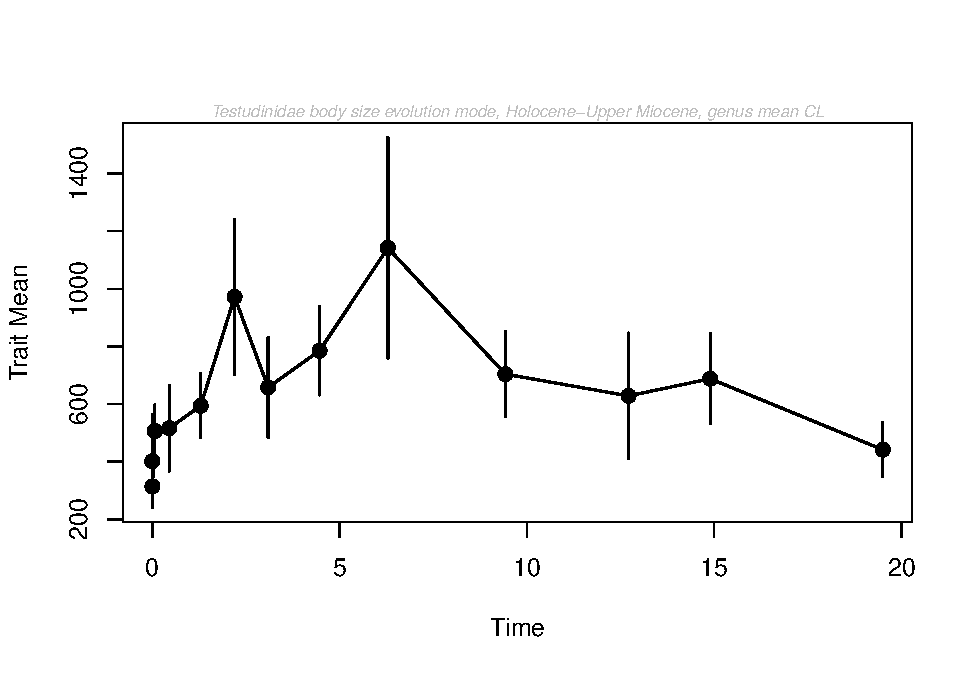
\includegraphics{MA_JJ_files/figure-latex/paleoTSAll-1.pdf}
	\caption[PaleoTS plot of complete data set]{Evolutionary trajectory of Testudinidae body size. Bars respresent standard errors of mean. The dashed line depicts the mean carapace length averaged across all time bins. The triangles indicate the Pleistocene/Pliocene and Pliocene/Miocene borders, respectively. Body size seems to continuously increase until the Upper Miocene, dip and go back up again in the Pliocene and steadily drop with onset of the Pleistocene.}
	\label{fig:pTSall}
\end{figure}

\begin{longtable}[]{@{}lrrrr@{}}
	\caption[Model fits for complete data set]{Model-fitting results for the complete data set. Stasis is the best although not very strongly supported model, followed by URW.}
	\phantomsection
	\label{tab:pTSallEM}\tabularnewline
	\toprule
	& logL & K & AICc & Akaike.wt\tabularnewline
	\midrule
	\endfirsthead
	\toprule
	& logL & K & AICc & Akaike.wt\tabularnewline
	\midrule
	\endhead
	GRW & -81.31790 & 2 & 167.9691 & 0.161\tabularnewline
	URW & -82.05721 & 1 & 166.5144 & 0.332\tabularnewline
	Stasis & -80.16802 & 2 & 165.6694 & 0.507\tabularnewline
	\bottomrule
\end{longtable}

\FloatBarrier
%__________________________________________________________________________

\subsubsection{continental dataset (excluding insular
	species)}\label{continental-excluding-insular-species}


\begin{longtable}[H]{@{}rrrr@{}}
	\caption[PaleoTS object of continental \T]{PaleoTS object of the continental data set. Mean Age (tt), sample size (nn), mean carapace lengths (mm) and variance (vv) are shown. Largest mean carapace length occurs in the Lower Pleistocene, followed closely by the Upper Miocene.}
	\phantomsection
	\label{tab:pTSC}\tabularnewline
	\toprule
	tt & nn & mm & vv\tabularnewline
	\midrule
	\endfirsthead
	\toprule
	tt & nn & mm & vv\tabularnewline
	\midrule
	\endhead
	0.00585 & 18 & 240.3544 & 11701.08\tabularnewline
	0.06885 & 6 & 397.4606 & 50619.39\tabularnewline
	0.45350 & 5 & 416.9341 & 200982.12\tabularnewline
	1.29350 & 7 & 346.8484 & 66240.07\tabularnewline
	2.19700 & 7 & 1103.1067 & 595507.93\tabularnewline
	3.09400 & 6 & 725.4156 & 414253.29\tabularnewline
	4.46600 & 6 & 771.3833 & 259173.08\tabularnewline
	6.28900 & 4 & 1054.4375 & 531455.93\tabularnewline
	9.42700 & 9 & 703.9570 & 195766.19\tabularnewline
	12.71400 & 6 & 628.3020 & 285258.36\tabularnewline
	14.89500 & 7 & 687.9619 & 169914.58\tabularnewline
	19.50000 & 9 & 441.5420 & 78467.65\tabularnewline
	\bottomrule
\end{longtable}

\begin{figure}[H]
	\centering
	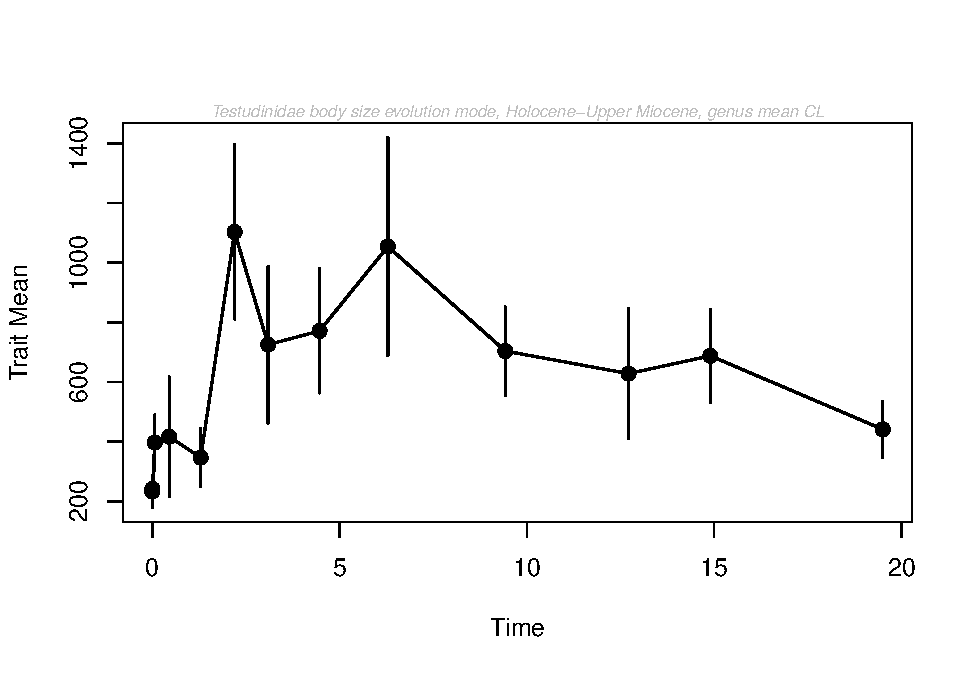
\includegraphics{MA_JJ_files/figure-latex/paleoTSC-1.pdf}
	\caption[PaleoTS plot of continental data set]{Evolutionary trajectory of Testudinidae body size on the continents. Bars respresent standard errors of mean. The dashed line depicts the mean carapace length averaged across all time bins. The triangles indicate the Pleistocene/Pliocene and Pliocene/Miocene borders, respectively. Body size seems to increase until the Upper Miocene, dip and go back up again in the Pliocene and steadily drop with onset of the Pleistocene.
	}
	\phantomsection
	\label{fig:pTSC}
\end{figure}

\begin{longtable}[]{@{}lrrrr@{}}
	\caption[Model fits for continental data set]{Model-fitting results for the continental data set. URW is the best although not very strongly supported model, followed by GRW.}
	\phantomsection
	\label{tab:pTSCEM}\tabularnewline
	\toprule
	& logL & K & AICc & Akaike.wt\tabularnewline
	\midrule
	\endfirsthead
	\toprule
	& logL & K & AICc & Akaike.wt\tabularnewline
	\midrule
	\endhead
	GRW & -82.26287 & 2 & 169.8591 & 0.300\tabularnewline
	URW & -83.12577 & 1 & 168.6515 & 0.548\tabularnewline
	Stasis & -82.93984 & 2 & 171.2130 & 0.152\tabularnewline
	\bottomrule
\end{longtable}


\FloatBarrier
%__________________________________________________________________________

\subsubsection{insular dataset (excluding
	continental)}\label{insular-excluding-continental}

\begin{longtable}[]{@{}rrrr@{}}
	\caption[PaleoTS object of insular \T]{PaleoTS object of the insular data set. Mean Age (tt), sample size (nn), mean carapace lengths (mm) and variance (vv) are shown. First records are from the Upper Miocene, where the largest mean carapace length occurs, followed by the Lower Pleistocene.}
	\phantomsection
	\label{tab:pTSI}\tabularnewline
	\toprule
	tt & nn & mm & vv\tabularnewline
	\midrule
	\endfirsthead
	\toprule
	tt & nn & mm & vv\tabularnewline
	\midrule
	\endhead
	0.00585 & 13 & 416.5655 & 80682.22\tabularnewline
	0.06885 & 4 & 727.5938 & 14997.58\tabularnewline
	0.45350 & 3 & 748.8333 & 142649.08\tabularnewline
	1.29350 & 6 & 829.6744 & 112964.44\tabularnewline
	2.19700 & 3 & 1178.3333 & 821158.33\tabularnewline
	3.09400 & 4 & 449.4375 & 27058.77\tabularnewline
	4.46600 & 2 & 826.1667 & 15196.06\tabularnewline
	6.28900 & 1 & 1850.0000 & 0.00\tabularnewline
	\bottomrule
\end{longtable}

\begin{figure}[H]
	\centering
	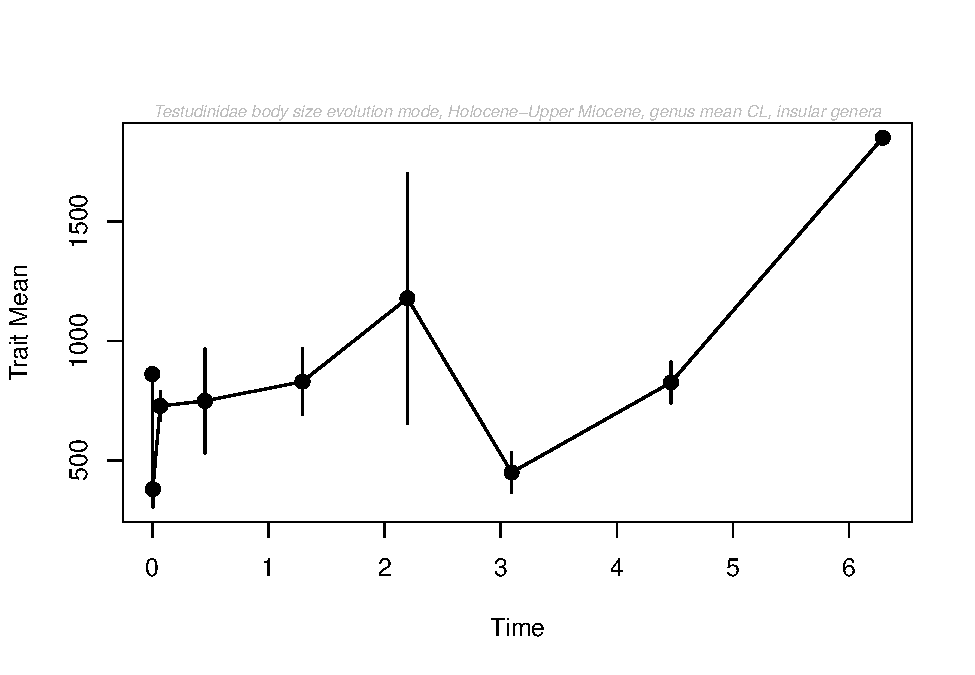
\includegraphics{MA_JJ_files/figure-latex/paleoTSI-1.pdf}
	\caption[PaleoTS plot of insular data set]{Evolutionary trajectory of Testudinidae body size on islands. Bars respresent standard errors of mean. The dashed line depicts the mean carapace length averaged across all time bins. The triangles indicate the Pleistocene/Pliocene and Pliocene/Miocene borders, respectively. Body size decreases during the Pliocene and goes back up again in the Lower Pleistocene, then drops slowly until it declines sharply in the Holocene.}
	\phantomsection
	\label{fig:pTSI}
\end{figure}

\begin{longtable}[]{@{}lrrrr@{}}
	\caption[Model fits for insular data set]{Model-fitting results for the insular data set. Stasis is the best supported model.
	}
	\phantomsection
	\label{tab:pTSIEM}\tabularnewline
	\toprule
	& logL & K & AICc & Akaike.wt\tabularnewline
	\midrule
	\endfirsthead
	\toprule
	& logL & K & AICc & Akaike.wt\tabularnewline
	\midrule
	\endhead
	GRW & -68.57344 & 2 & 143.5469 & 0\tabularnewline
	URW & -75.76576 & 1 & 154.1982 & 0\tabularnewline
	Stasis & -60.41581 & 2 & 127.2316 & 1\tabularnewline
	\bottomrule
\end{longtable}

\FloatBarrier
%__________________________________________________________________________

\subsubsection{per continent}\label{per-continent}

\paragraph{Europe, genera}\label{europe-genera}

When repeating the analysis for European taxa only, all three groups -- complete, continental and insular data -- are best described by stasis with a model support between 92\,-\,99\,\% (Fig. \ref{fig:pTSEu}, \ref{fig:pTSEuC}, \ref{fig:pTSEuI}; Tables \ref{tab:pTSEuEM}, \ref{tab:pTSEuCEM}, \ref{tab:pTSEuIEM}).

\begin{longtable}[]{@{}rrrr@{}}
	\caption[PaleoTS object of European \T]{PaleoTS object of European testudinids. Mean Age (tt), sample size (nn), mean carapace lengths (mm) and variance (vv) are shown. Largest mean carapace length occurs in the Lower Pliocene.}
	\phantomsection
	\label{tab:pTSEu}\tabularnewline
	\toprule
	tt & nn & mm & vv\tabularnewline
	\midrule
	\endfirsthead
	\toprule
	tt & nn & mm & vv\tabularnewline
	\midrule
	\endhead
	0.00585 & 2 & 148.8559 & 3338.406\tabularnewline
	0.06885 & 3 & 616.6667 & 138802.333\tabularnewline
	0.45350 & 3 & 377.8167 & 89203.953\tabularnewline
	1.29350 & 5 & 697.3717 & 218431.974\tabularnewline
	2.19700 & 2 & 895.0000 & 1110050.000\tabularnewline
	3.09400 & 3 & 453.3333 & 39433.333\tabularnewline
	4.46600 & 5 & 1215.8667 & 159317.256\tabularnewline
	6.28900 & 2 & 838.3750 & 875495.281\tabularnewline
	9.42700 & 6 & 800.0508 & 263434.389\tabularnewline
	12.71400 & 5 & 653.9625 & 351634.528\tabularnewline
	14.89500 & 5 & 772.0000 & 223154.375\tabularnewline
	19.50000 & 5 & 533.8533 & 183706.682\tabularnewline
	\bottomrule
\end{longtable}


\begin{figure}[H]
	\centering
	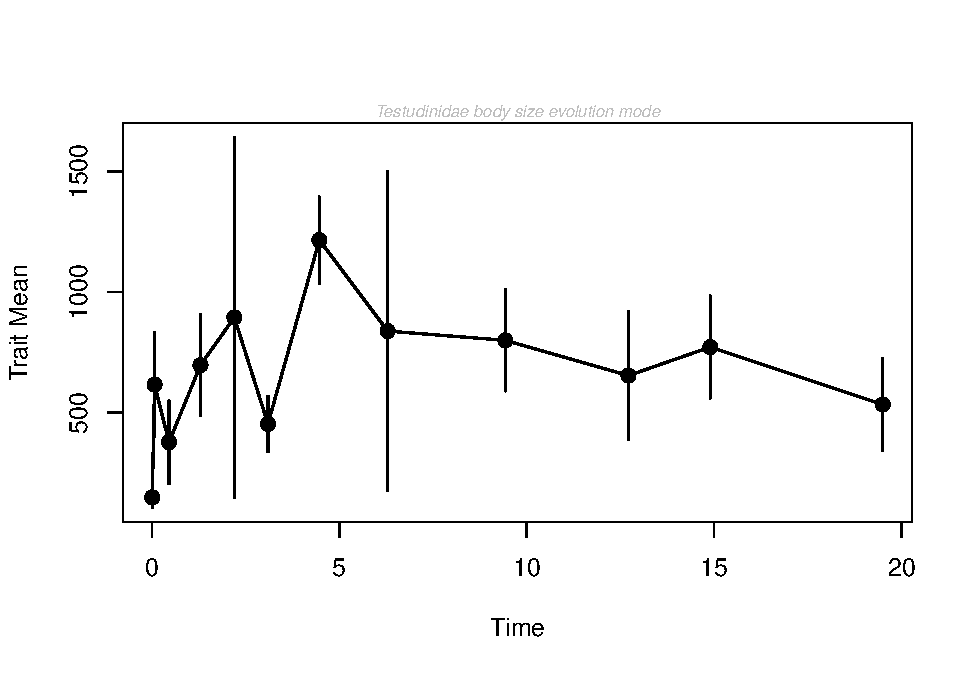
\includegraphics{MA_JJ_files/figure-latex/paleoTSEurope-1.pdf}
	\caption[PaleoTS plot of European \T]{Evolutionary trajectory of Testudinidae body size in Europe. Bars respresent standard errors of mean. The dashed line depicts the mean carapace length averaged across all time bins. The triangles indicate the Pleistocene/Pliocene and Pliocene/Miocene borders, respectively. Body size seems to increase until the Lower Pliocene and generally decline afterwards. However, body size shows two slight peaks, one at the beginnign and one at the end of the Pleistocene.}
	\phantomsection
	\label{fig:pTSEu}
\end{figure}

\begin{longtable}[]{@{}lrrrr@{}}
	\caption[Model fits for European \T]{Model-fitting results for European testudinids. Stasis is the best supported model.}
	\phantomsection
	\label{tab:pTSEuEM}\tabularnewline
	\toprule
	& logL & K & AICc & Akaike.wt\tabularnewline
	\midrule
	\endfirsthead
	\toprule
	& logL & K & AICc & Akaike.wt\tabularnewline
	\midrule
	\endhead
	GRW & -84.14010 & 2 & 173.7802 & 0.006\tabularnewline
	URW & -85.90727 & 1 & 174.2590 & 0.005\tabularnewline
	Stasis & -79.01365 & 2 & 163.5273 & 0.990\tabularnewline
	\bottomrule
\end{longtable}

\FloatBarrier
%__________________________________________________________________________



\paragraph{Eurasia,	genera}\label{eurasia-genera}


For Eurasia, the complete data set (Fig. \ref{fig:pTSEs}, Table \ref{tab:pTSEus}) and insular taxa are best described by stasis (Fig. \ref{fig:pTSEsI}, Table \ref{tab:pTSEsI}), with higher model supports than for the complete data set. Continental taxa are best described by an unbiased random walk (Fig. \ref{fig:pTSEsC}, Table \ref{tab:pTSEsC}), which reflects the results for the complete data set, although model support for Eurasian continental taxxa is even higher.


\begin{longtable}[]{@{}rrrr@{}}
	\caption[PaleoTS object of Eurasian \T]{PaleoTS object of the Eurasian testudinids. Mean Age (tt), sample size (nn), mean carapace lengths (mm) and variance (vv) are shown. Largest mean carapace length occurs from the Upper Miocene to the Lower Pliocene.}
	
	\phantomsection
	\label{tab:pTSEs}\tabularnewline
	\toprule
	tt & nn & mm & vv\tabularnewline
	\midrule
	\endfirsthead
	\toprule
	tt & nn & mm & vv\tabularnewline
	\midrule
	\endhead
	0.00585 & 6 & 210.8687 & 10460.89\tabularnewline
	0.06885 & 4 & 530.0000 & 122579.33\tabularnewline
	0.45350 & 3 & 377.8167 & 89203.95\tabularnewline
	1.29350 & 7 & 777.5579 & 162641.14\tabularnewline
	2.19700 & 5 & 909.6667 & 562217.22\tabularnewline
	3.09400 & 5 & 892.0000 & 381770.00\tabularnewline
	4.46600 & 6 & 1048.0556 & 296417.22\tabularnewline
	6.28900 & 3 & 1208.9167 & 849651.02\tabularnewline
	9.42700 & 6 & 800.0508 & 263434.39\tabularnewline
	12.71400 & 5 & 653.9625 & 351634.53\tabularnewline
	14.89500 & 5 & 772.0000 & 223154.38\tabularnewline
	19.50000 & 5 & 513.8533 & 162399.35\tabularnewline
	\bottomrule
\end{longtable}


\begin{figure}[H]
	\centering
	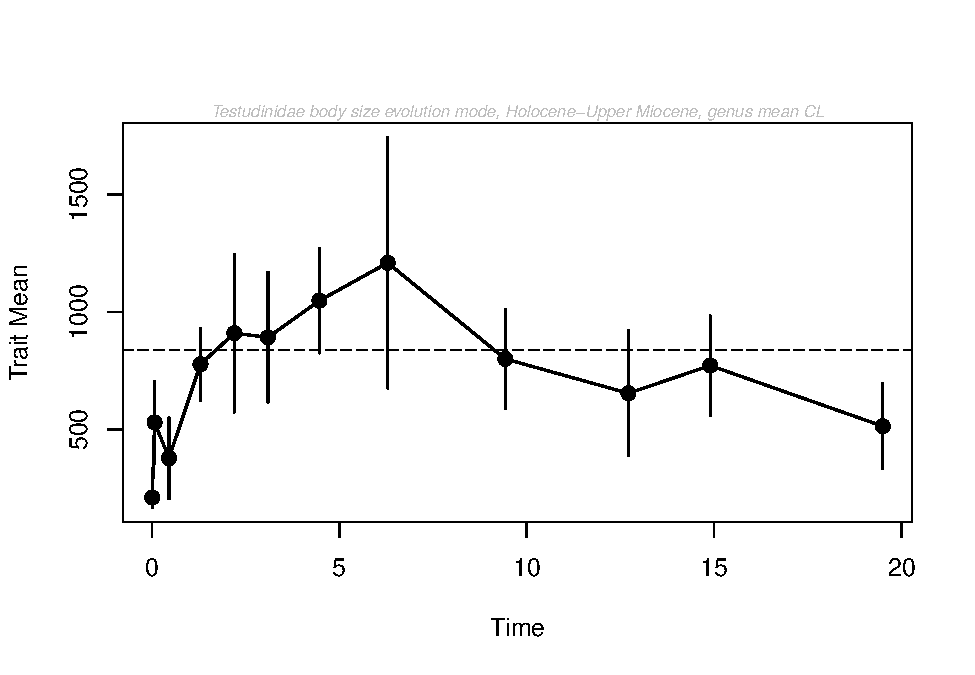
\includegraphics{MA_JJ_files/figure-latex/paleoTSEurasia-1.pdf}
	\caption[PaleoTS plot of Eurasian \T]{Evolutionary trajectory of Testudinidae body size in Eurasia. Bars respresent standard errors of mean. The dashed line depicts the mean carapace length averaged across all time bins. The triangles indicate the Pleistocene/Pliocene and Pliocene/Miocene borders, respectively. Body size seems to increase until the Upper Miocene and then decline continuously with only one slight peak during the Upper Pleistocene.}
	\phantomsection
	\label{tab:pTSEus}
\end{figure}

\begin{longtable}[]{@{}lrrrr@{}}
	\caption[Model fits for Eurasian \T]{Model-fitting results for Eurasian testudinids. Stasis is the best supported model.}
	\label{fig:pTSEs}\tabularnewline
	\toprule
	& logL & K & AICc & Akaike.wt\tabularnewline
	\midrule
	\endfirsthead
	\toprule
	& logL & K & AICc & Akaike.wt\tabularnewline
	\midrule
	\endhead
	GRW & -78.25066 & 2 & 162.0013 & 0.039\tabularnewline
	URW & -78.39530 & 1 & 159.2350 & 0.154\tabularnewline
	Stasis & -75.21099 & 2 & 155.9220 & 0.807\tabularnewline
	\bottomrule
\end{longtable}



\FloatBarrier
%__________________________________________________________________________

